\ifnum \Version=1
\question[1] You do not need to show your work for this question. Consider the nonlinear system below.
\begin{align*}
    \dxdt &= (x-1)(y-5) , \qquad \dydt = y-x^2-1
\end{align*}
How many critical points does the system have? \framebox{\strut\hspace{1cm}}
\ifnum \Solutions=1 {\color{DarkBlue} \\[12pt] 
For a point to critical point, we need $x' = y' = 0$. If $x'$ is zero, then either $x=1$ or $y=5$. Likewise if $y'=0$ then $y=x^2+1$. The curves are shown below. The green lines are the x nullclines, and the red curve is the y nullcline. There are exactly three critical points. 
    \begin{center}
    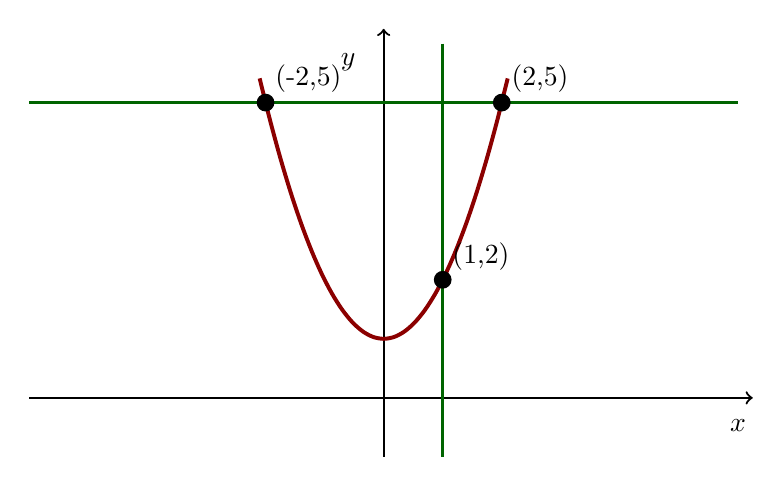
\begin{tikzpicture}[scale=0.75]
    \draw[thick, ->] (-6, 0) -- (6.25, 0);
    \draw[thick, ->] (0, -1) -- (0, 6.25);
    \node[overlay, below] at (6, -0.2) {$x$};
    \node[overlay, below] at (-0.6, 6) {$y$};   
    \draw[very thick,DarkGreen, -] (1, 6) -- (1, -1);        
    \draw[very thick,DarkGreen, -] (-6, 5) -- (6, 5);   
    \draw[DarkRed, line width = 0.50mm]   plot[smooth,domain=-2.1:2.1] (\x, {\x*\x+1});
    \filldraw[black] (2,5) circle (4pt) node[anchor=south west]{(2,5)};
    \filldraw[black] (-2,5) circle (4pt) node[anchor=south west]{(-2,5)};
    \filldraw[black] (1,2) circle (4pt) node[anchor=south west]{(1,2)};
    \end{tikzpicture}
    \end{center}         
} 
\else 
\vspace{3cm}
\fi    
\fi 


\ifnum \Version=2
\question[1] You do not need to show your work for this question. Consider the nonlinear system below.
\begin{align*}
    \dxdt &= (y-1)(y-5)(x-1) , \qquad \dydt = y-x^2-1
\end{align*}
How many critical points does the system have? \framebox{\strut\hspace{1cm}}
\ifnum \Solutions=1 {\color{DarkBlue} \\[12pt] 
For a point to critical point, we need $x' = y' = 0$. If $x'$ is zero, then either $x=1$, $y=1$ or $y=5$. Likewise if $y'=0$ then $y=x^2+1$. The curves are shown below. The green lines are the x nullclines, and the red curve is the y nullcline. There are exactly four critical points. 
    \begin{center}
    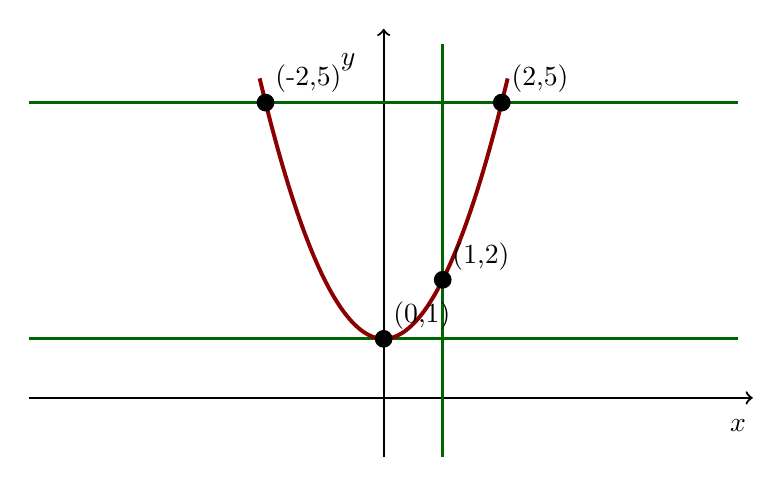
\begin{tikzpicture}[scale=0.75]
    \draw[thick, ->] (-6, 0) -- (6.25, 0);
    \draw[thick, ->] (0, -1) -- (0, 6.25);
    \node[overlay, below] at (6, -0.2) {$x$};
    \node[overlay, below] at (-0.6, 6) {$y$};   
    \draw[very thick,DarkGreen, -] (-6, 1) -- (6, 1);   
    \draw[very thick,DarkGreen, -] (-6, 5) -- (6, 5);   
    \draw[very thick,DarkGreen, -] (1, -1) -- (1, 6);   
    \draw[DarkRed, line width = 0.50mm]   plot[smooth,domain=-2.1:2.1] (\x, {\x*\x+1});
    \filldraw[black] (2,5) circle (4pt) node[anchor=south west]{(2,5)};
    \filldraw[black] (1,2) circle (4pt) node[anchor=south west]{(1,2)};
    \filldraw[black] (-2,5) circle (4pt) node[anchor=south west]{(-2,5)};
    \filldraw[black] (0,1) circle (4pt) node[anchor=south west]{(0,1)};
    \end{tikzpicture}
    \end{center}         
} 
\else 
\vspace{3cm}
\fi    
\fi 



\ifnum \Version=3
\question[1] You do not need to show your work for this question. Consider the nonlinear system below.
\begin{align*}
    \dxdt &= (x-1)(y-5) , \qquad \dydt = y-x^2-1
\end{align*}
How many critical points does the system have? \framebox{\strut\hspace{1cm}}
\ifnum \Solutions=1 {\color{DarkBlue} \\[12pt] 
For a point to critical point, we need $x' = y' = 0$. If $x'$ is zero, then either $x=1$ or $y=5$. Likewise if $y'=0$ then $y=x^2+1$. The curves are shown below. The green lines are the x nullclines, and the red curve is the y nullcline. There are exactly three critical points. 
    \begin{center}
    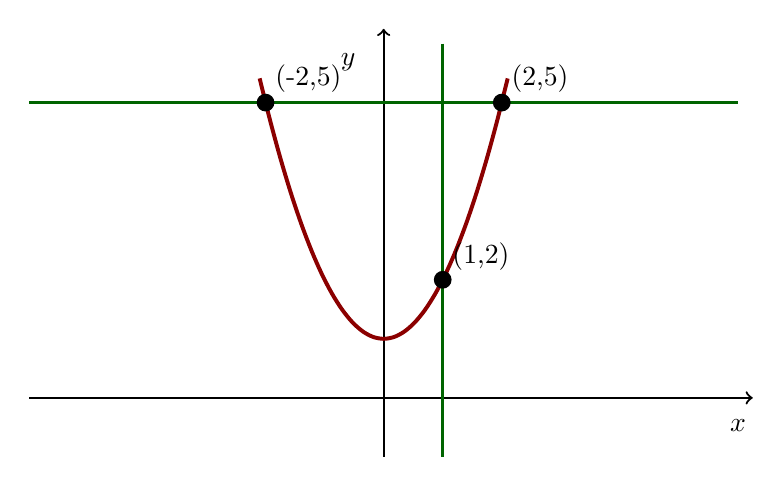
\begin{tikzpicture}[scale=0.75]
    \draw[thick, ->] (-6, 0) -- (6.25, 0);
    \draw[thick, ->] (0, -1) -- (0, 6.25);
    \node[overlay, below] at (6, -0.2) {$x$};
    \node[overlay, below] at (-0.6, 6) {$y$};   
    \draw[very thick,DarkGreen, -] (1, 6) -- (1, -1);        
    \draw[very thick,DarkGreen, -] (-6, 5) -- (6, 5);   
    \draw[DarkRed, line width = 0.50mm]   plot[smooth,domain=-2.1:2.1] (\x, {\x*\x+1});
    \filldraw[black] (2,5) circle (4pt) node[anchor=south west]{(2,5)};
    \filldraw[black] (-2,5) circle (4pt) node[anchor=south west]{(-2,5)};
    \filldraw[black] (1,2) circle (4pt) node[anchor=south west]{(1,2)};
    \end{tikzpicture}
    \end{center}         
} 
\else 
\vspace{1cm}
\fi    
\fi 


\ifnum \Version=4
\question[1] You do not need to show your work for this question. Consider the nonlinear system below.
\begin{align*}
    \dxdt &= (y-4)(x-1) , \qquad \dydt = y-x^2
\end{align*}
Where are the critical points of this system located? % \framebox{\strut\hspace{5cm}}
\ifnum \Solutions=1 {\color{DarkBlue} \\[12pt] 
For a point to critical point, we need $x' = y' = 0$. If $x'$ is zero, then either $x=1$, or $y=4$. Likewise if $y'=0$ then $y=x^2$. The curves are shown below. The green lines are the x nullclines, and the red curve is the y nullcline. There are exactly three critical points. We care not for the points where green crosses green. 
    \begin{center}
    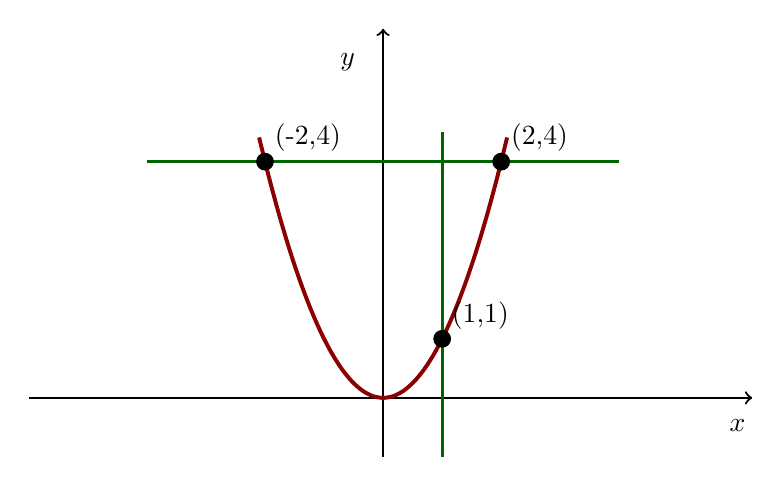
\begin{tikzpicture}[scale=0.75]
    \draw[thick, ->] (-6, 0) -- (6.25, 0);
    \draw[thick, ->] (0, -1) -- (0, 6.25);
    \node[overlay, below] at (6, -0.2) {$x$};
    \node[overlay, below] at (-0.6, 6) {$y$};   
    \draw[very thick,DarkGreen, -] (1, -1) -- (1, 4.5);   
    \draw[very thick,DarkGreen, -] (-4, 4) -- (4, 4);   
    \draw[DarkRed, line width = 0.50mm]   plot[smooth,domain=-2.1:2.1] (\x, {\x*\x});
    \filldraw[black] (1,1) circle (4pt) node[anchor=south west]{(1,1)};
    \filldraw[black] (2,4) circle (4pt) node[anchor=south west]{(2,4)};
    \filldraw[black] (-2,4) circle (4pt) node[anchor=south west]{(-2,4)};
    \end{tikzpicture}
    \end{center}         
} 
\else 
\vspace{3cm}
\fi    
\fi 



\ifnum \Version=6
\newpage
\question[3] You do not need to show your work for this question. Consider the nonlinear system below.
\begin{align*}
    \dxdt &= x(4-2x-y) , \qquad \dydt = y(2-2x-y)
\end{align*}
You can assume that $x$ and $y$ represent populations, so $x\ge0$ and $y\ge0$. 
\begin{parts}
    \part Write down the equations of the lines that correspond to where solution curves are horizontal. 
    
    \ifnum \Solutions=1 {\color{DarkBlue} 
    \textbf{Solutions:} horizontal where $y'=0$, which occurs on the lines $y=0$ and $y=2-2x$. 
    } 
    \else 
    \vspace{2cm}
    \fi
    \part Where are the critical points of this system located? 

    \ifnum \Solutions=1 {\color{DarkBlue} 
    \textbf{Solutions:} by inspection the only CPs are at $(0,0)$, $(0,2)$, $(2,0)$. 
    } 
    \else 
    \vspace{4cm}
    \fi
    \part Sketch the nullclines of the system on the axes below. Clearly indicate the critical points. 
    \ifnum \Solutions=1 {\color{DarkBlue} \\[12pt] 
        Green lines are the $x-$nullclines, red lines are the $y-$nullclines.
        \begin{center}
        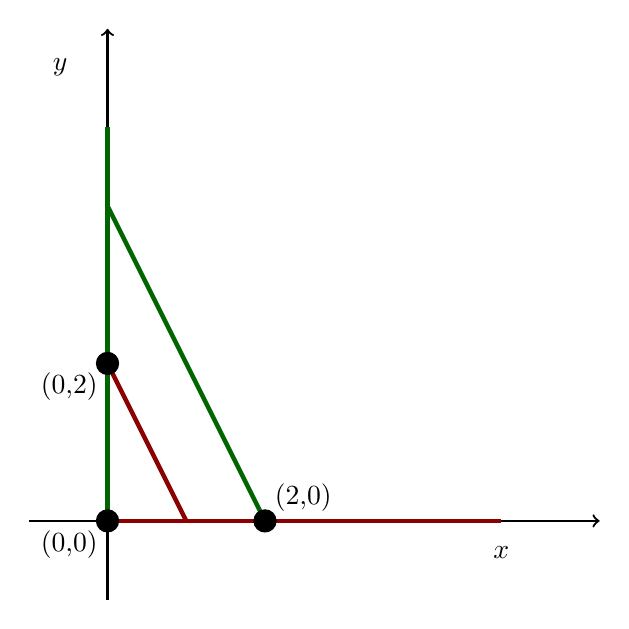
\begin{tikzpicture}[scale=1]
        \draw[thick, ->] (-1, 0) -- (6.25, 0);
        \draw[thick, ->] (0, -1) -- (0, 6.25);
        \node[overlay, below] at (5, -0.2) {$x$};
        \node[overlay, below] at (-0.6, 6) {$y$};   
        \draw[ultra thick,DarkRed, -] (0, 0) -- (5, 0);        
        \draw[ultra thick,DarkGreen, -] (0,4) -- (2, 0);   
        \draw[ultra thick,DarkRed, -] (0, 2) -- (1, 0);        
        \draw[ultra thick,DarkGreen, -] (0, 0) -- (0, 5);      
        \filldraw[black] (0,0) circle (4pt) node[anchor=north east]{(0,0)};
        \filldraw[black] (0,2) circle (4pt) node[anchor=north east]{(0,2)};
        \filldraw[black] (2,0) circle (4pt) node[anchor=south west]{(2,0)};
        \end{tikzpicture}
        \end{center}            
        } 
        \else 
        \begin{center}
        \begin{tikzpicture}[scale=0.65]
        \draw[very thick, ->] (-0.5, 0) -- (6.25, 0);
        \draw[very thick, ->] (0, -0.5) -- (0, 6.25);
        \node[overlay, below] at (6, -0.2) {$x$};
        \node[overlay, below] at (-0.6, 6) {$y$};        
        \end{tikzpicture}
        \end{center}    
    \fi
\end{parts}
\fi




\ifnum \Version=7
\newpage
\question[3] You do not need to show your work for this question. Consider the nonlinear system below.
\begin{align*}
    \dxdt &= x(6-2x-y) , \qquad \dydt = y(2-2x-y)
\end{align*}
You can assume that $x$ and $y$ represent populations, so $x\ge0$ and $y\ge0$. 
\begin{parts}
    \part Write down the equations of the lines that correspond to where solution curves are vertical. 
    
    \ifnum \Solutions=1 {\color{DarkBlue} 
    \textbf{Solutions:} horizontal where $x'=0$, which occurs on the lines $x=0$ and $y=6-2x$. 
    } 
    \else 
    \vspace{2cm}
    \fi
    \part Where are the critical points of this system located? 

    \ifnum \Solutions=1 {\color{DarkBlue} 
    \textbf{Solutions:} by inspection the only CPs are at $(0,0)$, $(0,2)$, $(3,0)$. 
    } 
    \else 
    \vspace{6cm}
    \fi
    \part Sketch the nullclines of the system on the axes below. Clearly indicate the critical points. 
        \ifnum \Solutions=1 {\color{DarkBlue} \\[12pt] 
        Green lines are the $x-$nullclines, red lines are the $y-$nullclines.
        \begin{center}
        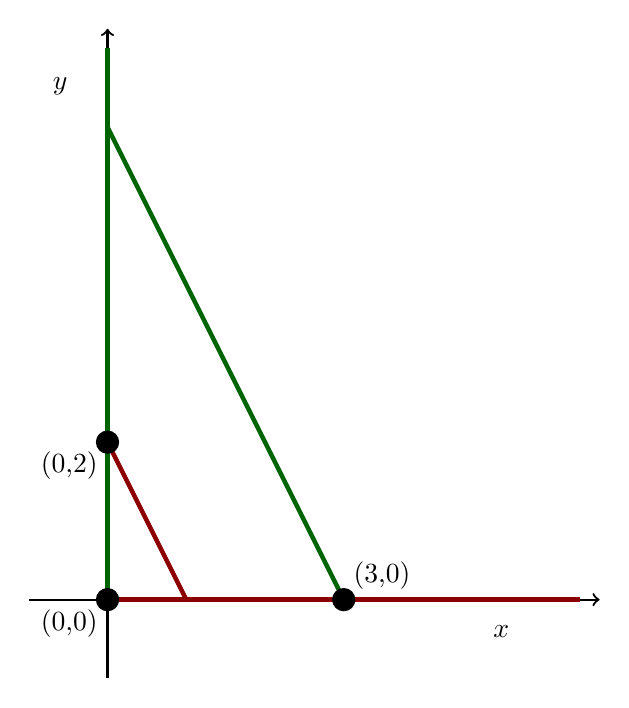
\begin{tikzpicture}[scale=1]
        \draw[thick, ->] (-1, 0) -- (6.25, 0);
        \draw[thick, ->] (0, -1) -- (0, 7.25);
        \node[overlay, below] at (5, -0.2) {$x$};
        \node[overlay, below] at (-0.6, 6.75) {$y$};   
        \draw[ultra thick,DarkRed, -] (0, 0) -- (6, 0);        
        \draw[ultra thick,DarkGreen, -] (0,6) -- (3, 0);   
        \draw[ultra thick,DarkRed, -] (0, 2) -- (1, 0);        
        \draw[ultra thick,DarkGreen, -] (0, 0) -- (0, 7);      
        \filldraw[black] (0,0) circle (4pt) node[anchor=north east]{(0,0)};
        \filldraw[black] (0,2) circle (4pt) node[anchor=north east]{(0,2)};
        \filldraw[black] (3,0) circle (4pt) node[anchor=south west]{(3,0)};
        \end{tikzpicture}
        \end{center}            
        } 
        \else 
        \begin{center}
        \begin{tikzpicture}[scale=0.65]
        \draw[very thick, ->] (-0.5, 0) -- (6.25, 0);
        \draw[very thick, ->] (0, -0.5) -- (0, 6.25);
        \node[overlay, below] at (6, -0.2) {$x$};
        \node[overlay, below] at (-0.6, 6) {$y$};
        \end{tikzpicture}
        \end{center}    
    \fi
\end{parts}
\fi